% Created by Jim Finnis
% Date Wed Feb 24 13:35:30 2021


\section{Introduction}
These notes provide some architectural details for PCOT to help
maintainers. I'll try to keep them up to date.

PCOT is based around a directed graph of nodes which perform
transformations of data. For this reason, the nodes are sometimes
called ``transforms'' and are represented by the \texttt{XForm} class
in the code.
Usually the data in question is an image, or rather an ``image cube'':
these have an arbitrary number of channels, not just the typical
RGB or greyscale. However, the data can be anything at all --- it depends
on the node. There is some typechecking when constructing the graph:
for exampel, you can't connect a ``rectangle'' output to an ``image'' input.
The entire application is shown in Fig.~\ref{app.png}. On the right
is a ``palette'' from which nodes can be selected to add to the graph,
while on the left
is an area which can show controls for each node in the graph, while
in the centre-right is the graph itself. This is shown in more detail
in Fig.~\ref{graph.png}.

\begin{figure}[ht]
\center
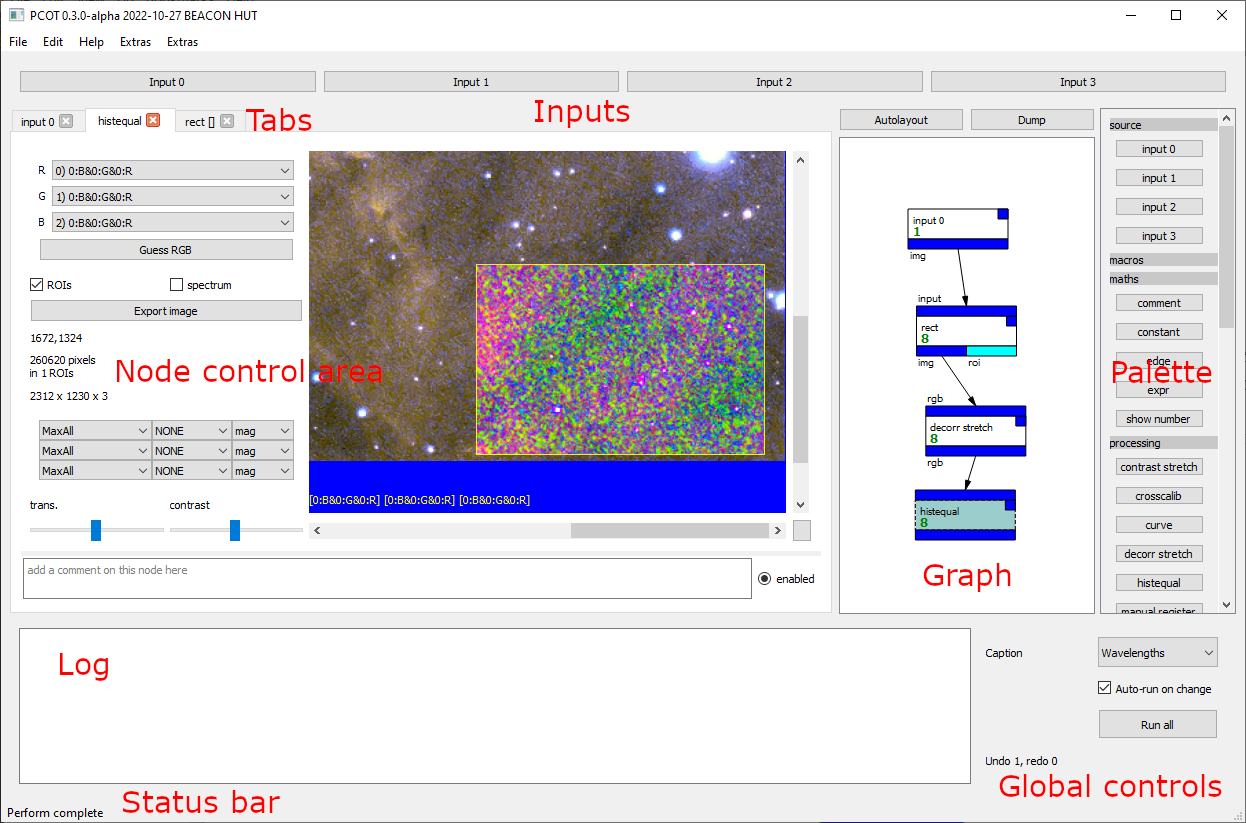
\includegraphics[width=5in]{app.png}
\caption{The PCOT application}
\label{app.png}
\end{figure}

\clearpage
This will take an RGB image from a file, perform a decorrelation stretch,
and then a histogram equalisation on the three channels. It will
only do this to a rectangular portion of the image (defined by the
\texttt{rect} node), annotating the region with some text defined in
the \texttt{rect} node's controls. The control region is currently
showing the output of the histogram equalisation.

\begin{figure}[ht]
\center
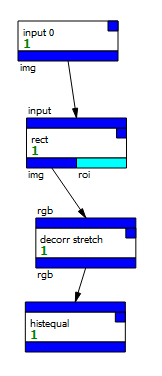
\includegraphics[width=1in]{graph.png}
\caption{An example graph}
\label{graph.png}
\end{figure}


